\chapter{وراثة النماء وتطور الشكل}\label{ch:b3:developmental-genetics}

بيضة ذبابة الفاكهة طولها نصف ميليمتر، وفي الساعات الثلاث
التالية للإلقاح، قبل أن يتكوّن غشاء خلوي واحد بين نُواها
الستة آلاف، تقرر أي طرف سيكون الرأس وأيهما الذنب، وأين تقع
كل قطعة من أربع عشرة قطعة، وأيها سيحمل أرجلًا أو أجنحة أو
قرون استشعار. وتفعل ذلك ببضع عشرات من المورّثات، تُشغَّل في
تراتب من خطوط تزداد دقة، كل خط يُقرأ من تراكيز نواتج الخطوط
التي قبله. وفي عام 1980 فحص عالمان شابان في هايدلبرغ آلاف
الذبابات الطافرة بحثًا عن يرقات ناقصة الأجزاء أو مضاعفتها،
فوجدا التراتب كله: مورّثات يحذف فقدها كتلة من القطع،
ومورّثات يحذف فقدها قطعة بعد أخرى، ومورّثات يقلب فقدها كل
قطعة رأسًا على عقب. وفتح عمل السنة نفسها على مورّثة تحوّل
القطعة الثالثة في ذبابة إلى نسخة من الثانية --- فتعطيها
أربعة أجنحة، كما كان لأسلافها --- مجموعةً من المورّثات
السيدة تبيّن أنها تقع بالترتيب نفسه على صبغيات الفأر
والإنسان، وتؤدي العمل نفسه. وهذا الفصل عن كيف يحسب جنين
هندسته هو، وكيف تبني بضع مئات من المورّثات المنظِّمة كل جسد
حيواني، وكيف أنتج تغيير متى تعمل وأين تنوعَ الشكل الحيواني.

\section{إحداثيات الذبابة}

\begin{definition}[تراتب التقطيع]\label{def:b3:developmental-genetics:hierarchy}
\index{مورّثة أثر أمومي}\index{مورّثة فجوية}\index{مورّثة زوجية القاعدة}\index{مورّثة قطبية القطعة}\index{أديم أرومي مدمج}
ينمو جنين \emph{Drosophila} في انقساماته النووية الثلاثة عشر
الأولى \emph{أديمًا أروميًا مدمجًا}، أي خلية واحدة تتشارك
نُواها عصارة واحدة، فتنتشر البروتينات بحرية من حيث تُصنع.
وأربعة تدرجات تضعها خلايا الأم تحدد المحاور: فرسول
\emph{bicoid} مربوط عند القطب الأمامي وبروتينه ينتشر راجعًا
فيكوّن تدرجًا أسّيًا من الرأس إلى الذنب؛ ورسول \emph{nanos}
عند القطب الخلفي يصنع التدرج المرآتي؛ ورسولا
\emph{hunchback} و\emph{caudal} منتظمان، غير أن بروتين Bicoid
يكبت ترجمة \emph{caudal} ويكبت Nanos ترجمة
\emph{hunchback}، فيكوّن بروتيناهما تدرجين أيضًا. وهذه
النواتج \emph{ذات الأثر الأمومي}، التي يتوقف نمطها الظاهري
الطافر على نمط الأم الوراثي لا الجنين، تشغّل \emph{المورّثات
الفجوية} (\emph{hunchback}، و\emph{Krüppel}، و\emph{knirps}،
و\emph{giant}) في أشرطة عريضة، كل واحدة تستجيب لمدى من تركيز
Bicoid وتكبت جاراتها؛ وتشغّل البروتينات الفجوية، بتوافيقها،
\emph{المورّثات الزوجية القاعدة} (\emph{even-skipped}،
و\emph{fushi tarazu}، و\emph{hairy}) في سبعة خطوط لكل منها،
متناوبة؛ وتشغّل البروتينات الزوجية القاعدة \emph{مورّثات
قطبية القطعة} (\emph{engrailed}، و\emph{wingless}،
و\emph{hedgehog}) في أربعة عشر خطًا، خط لكل قطعة، تحدد أمام
كل قطعة وخلفها وتُصان، بعد تكوّن الخلايا، بالإشارة بينها.
ثلاث ساعات، وأربع طبقات، من تدرج واحد إلى أربع عشرة قطعة ---
وأسماء الطافرات تسجّل الفحص: فالمورّثة \emph{hunchback} تفتقر إلى
الصدر، و\emph{Krüppel} (``الكسيح'') إلى الوسط،
و\emph{fushi tarazu} (``القطع غير كافية'') إلى قطعة بعد أخرى،
و\emph{hedgehog} له مرج من الأشواك.
\end{definition}

\begin{omfigure}
\begin{tikzpicture}[every node/.style={font=\scriptsize}, >=stealth]
  \foreach \y/\lab/\n in {0/{أمومي: تدرج Bicoid}/1, -1.3/{مورّثات فجوية: 4 أشرطة عريضة}/2, -2.6/{مورّثات زوجية القاعدة: 7 خطوط}/3, -3.9/{قطبية القطعة: 14 خطًا}/4} {
    \draw[thick, gray!60] (0,\y) ellipse (3.6 and 0.5);
    \node[left, align=right] at (-3.8,\y) {\lab};
  }
  % bicoid gradient shading
  \begin{scope}
    \clip (0,0) ellipse (3.6 and 0.5);
    \shade[left color=omDef!80, right color=omDef!2] (-3.6,-0.5) rectangle (3.6,0.5);
  \end{scope}
  \node[right, font=\tiny] at (3.7,0) {الأمام مرتفع};
  % gap bands
  \begin{scope}
    \clip (0,-1.3) ellipse (3.6 and 0.5);
    \fill[omDef!50] (-3.4,-1.8) rectangle (-1.6,-0.8); \fill[omThm!40] (-1.4,-1.8) rectangle (0.2,-0.8); \fill[omMeth!40] (0.4,-1.8) rectangle (1.7,-0.8); \fill[omProp!45] (1.9,-1.8) rectangle (3.4,-0.8);
  \end{scope}
  \node[font=\tiny] at (-2.5,-1.3) {\emph{hb}}; \node[font=\tiny] at (-0.6,-1.3) {\emph{Kr}}; \node[font=\tiny] at (1.05,-1.3) {\emph{kni}}; \node[font=\tiny] at (2.65,-1.3) {\emph{gt}};
  % pair-rule stripes
  \begin{scope}
    \clip (0,-2.6) ellipse (3.6 and 0.5);
    \foreach \i in {0,...,6} { \fill[omThm!50] ({-3.1+\i*0.9},-3.1) rectangle ({-2.75+\i*0.9},-2.1); }
  \end{scope}
  \node[right, font=\tiny] at (3.7,-2.6) {\emph{eve}، قطعة بعد أخرى};
  % segment polarity stripes
  \begin{scope}
    \clip (0,-3.9) ellipse (3.6 and 0.5);
    \foreach \i in {0,...,13} { \fill[omProp!60] ({-3.25+\i*0.47},-4.4) rectangle ({-3.1+\i*0.47},-3.4); }
  \end{scope}
  \node[right, font=\tiny] at (3.7,-3.9) {\emph{en}: واحد لكل قطعة};
  \foreach \y in {-0.55,-1.85,-3.15} { \draw[->, thick] (0,\y) -- (0,\y-0.2); }
  \node[below, align=center, font=\tiny] at (0,-4.5) {كل طبقة تقرأ تراكيز الطبقة التي فوقها؛\\ثلاث ساعات من تدرج واحد إلى أربع عشرة قطعة};
\end{tikzpicture}

{\small تراتب التقطيع. يُقرأ تدرج أمومي في أربعة أشرطة
مورّثية فجوية؛ والبروتينات الفجوية، بتوافيقها، في سبعة خطوط
زوجية القاعدة؛ وتلك في أربعة عشر خطًا لقطبية القطع. وكل خط
حدٌّ يُرسم حيث يعبر تركيزٌ عتبةً.}
\end{omfigure}

\begin{theorem}[تدرج مورفوجيني من التركيب والانتشار والاضمحلال]\label{thm:b3:developmental-genetics:gradient}
\index{مورفوجين}\index{معلومة موضعية}\index{نموذج العلم الفرنسي}\index{طول الاضمحلال}
بروتين يُصنع عند طرف نسيج بمعدل $J$ (في وحدة المساحة)،
وينتشر بمعامل $D$، ويُهدم بثابت معدل $k$، يبلغ حالة مستقرة
يخضع فيها تركيزه على امتداد المحور $x$ للعلاقة
\[
D\,\frac{\mathrm{d}^{2}c}{\mathrm{d}x^{2}} - k\,c = 0,
\qquad c(x) = c_{0}\,\mathrm{e}^{-x/\lambda}, \qquad \lambda = \sqrt{D/k},
\quad c_{0} = \frac{J}{\sqrt{Dk}} .
\]
و\emph{\omterm{thm:b3:developmental-genetics:gradient}{طول الاضمحلال}} $\lambda$ يحدد مدى التدرج؛ وتقرأ الخلية
موضعها بمقارنة $c$ بعتبات --- أي \emph{العلم الفرنسي} عند
وولبرت (1969): فوق $T_{1}$ أزرق، وبين $T_{1}$ و$T_{2}$ أبيض،
ودونه أحمر --- ويقع حد العتبة $T$ عند
$x_{T} = \lambda\ln(c_{0}/T)$. ونتيجتان: أن مضاعفة المنبع تزيح
كل حد إلى الوراء بالمقدار نفسه $\lambda\ln 2$، وأن خطأً نسبيًا
$\delta c/c$ في قراءة التركيز هو خطأ موضعي
$\delta x = \lambda\,\delta c/c$، فلا يقدر تدرج على وضع حدّ
في حدود خلية واحدة إلا إذا قرأته الخلايا في حدود بضع في
المئة. ولبروتين Bicoid طول اضمحلال $\lambda \approx \qty{100}{\micro m}$
في بيضة طولها \qty{500}{\micro m}: فيمتد التدرج على عامل
$\mathrm{e}^{5}
\approx 150$، ويقع حد \emph{hunchback} في منتصف
البيضة حيث يكون Bicoid قد هبط إلى نحو جزء من اثني عشر من
ذروته.
\end{theorem}
\begin{proof}
الحفظ في شريحة بين $x$ و$x + \mathrm{d}x$: فالتدفق الانتشاري
الصافي الداخل $D\,\partial^{2}c/\partial x^{2}$ يوازن
الهدم $kc$ في الحالة المستقرة، فتنتج المعادلة؛ والحل المحدود
عند $x \to \infty$ هو الأسّي الخامد عند
$\lambda^{2} = D/k$. وأما المنبع: فالدفق الانتشاري عند $x = 0$، وهو $-D\,
c'(0) = Dc_{0}/\lambda$، يساوي $J$، فيكون $c_{0} = J\lambda/D =
J/\sqrt{Dk}$. وأما العتبة: فإن $c_{0}\mathrm{e}^{-x_{T}/\lambda} = T$ يعطي
$x_{T}$؛ ومضاعفة $c_{0}$ تضيف $\lambda\ln 2$ إلى كل $x_{T}$
بصرف النظر عن $T$. وأما الخطأ: فباشتقاق $x_{T} = \lambda\ln(c_{0}/c)$
نجد $\delta x = -\lambda\,\delta c/c$. وتُبلَغ الحالة المستقرة
على مقياس زمني $1/k$، وهو لبروتين Bicoid (\qty{50}{min}) مقارب
للساعتين المتاحتين، فيُقرأ التدرج وهو لا يزال يستقر.
\end{proof}

\begin{omfigure}
\begin{tikzpicture}
\begin{axis}[
  width=0.7\linewidth, height=5.6cm,
  axis x line=bottom, axis y line=left,
  xmin=0, xmax=500, ymin=0, ymax=1.05,
  xlabel={المسافة عن القطب الأمامي (\unit{\micro m})}, ylabel={Bicoid، نسبيًا},
  xlabel style={font=\small, at={(axis description cs:0.5,-0.12)}, anchor=north}, ylabel style={font=\small},
  tick label style={font=\small}, xtick={0,100,250,400,500}, ytick={0.08,0.3,0.6,1},
  yticklabels={0.08,0.3,0.6,1},
  clip=false,
]
\fill[omDef!15] (axis cs:0,0) rectangle (axis cs:120,1.05);
\fill[gray!8] (axis cs:120,0) rectangle (axis cs:250,1.05);
\fill[omThm!12] (axis cs:250,0) rectangle (axis cs:500,1.05);
\addplot[very thick, omDef, domain=0:500, samples=100] {exp(-x/100)};
\addplot[thick, omDef!50, dashed, domain=66:500, samples=100] {2*exp(-x/100)};
\draw[dashed, gray] (axis cs:0,0.3) -- (axis cs:120,0.3) -- (axis cs:120,0);
\draw[dashed, gray] (axis cs:0,0.08) -- (axis cs:250,0.08) -- (axis cs:250,0);
\node[font=\scriptsize, anchor=south] at (axis cs:60,1.0) {الرأس};
\node[font=\scriptsize, anchor=south] at (axis cs:185,1.0) {الصدر};
\node[font=\scriptsize, anchor=south] at (axis cs:375,1.0) {البطن};
\node[font=\scriptsize, omDef, anchor=west] at (axis cs:255,0.35) {$c = c_{0}\,\mathrm{e}^{-x/\lambda}$، $\lambda = \qty{100}{\micro m}$};
\node[font=\scriptsize, omDef!70!black, anchor=west, align=left] at (axis cs:255,0.62) {المتقطع: المنبع مضاعَفًا ---\\وكل حد ينزاح $\lambda\ln 2 = \qty{69}{\micro m}$};
\node[font=\scriptsize, gray, anchor=north east] at (axis cs:118,0.29) {$T_{1}$};
\node[font=\scriptsize, gray, anchor=south west] at (axis cs:300,0.09) {$T_{2}$: \emph{hunchback} مطفأة};
\end{axis}
\end{tikzpicture}

{\small العلم الفرنسي يرسمه أسّي. عتبات على تدرج واحد تقسم
البيضة إلى مناطق؛ ومنبع أقوى يحرّك الحدود كلها إلى الوراء
بالمسافة نفسها، وهو ما تُظهره أجنّة من أمهات لديهن نسخ
إضافية من \emph{bicoid}.}
\end{omfigure}

\begin{proof}[شواهد]
أطعمت نوسلاين-فولهارد وفيشاوس (1980) ذبابًا مطفِّرًا، وربّيا
الخلف حتى تخالص الزيجة، ونظرا في قشيرات نحو \num{27000} يرقة
ميتة تحت المجهر بحثًا عن نمط ناقص أو مكرَّر: فوجدا نحو مئة
وعشرين مورّثة، مرتبةً بأنماطها الظاهرية في أصناف الفجوية
والزوجية القاعدة وقطبية القطعة --- أي تراتب مرئي قبل أن
يُعرف أي جزيء. ثم صبغ دريفر ونوسلاين-فولهارد (1988) أجنّةً
لبروتين Bicoid فرأيا التدرج الأسّي من القطب الأمامي؛ وكانت
أجنّة الأمهات ذوات النسخة أو النسختين أو الأربع أو الست ذات
تدرجات متناسبة الارتفاع، وانتقلت طية الرأس وحدّ
\emph{hunchback} خلفيًا مع الجرعة، كما يتنبأ نموذج العتبة
وبمقدار يقارب $\lambda\ln 2$ لكل مضاعفة كما يقتضي. وحقنُ
رسول \emph{bicoid} في وسط بيضة أنتج رأسًا هناك.
\end{proof}

\begin{omfigure}
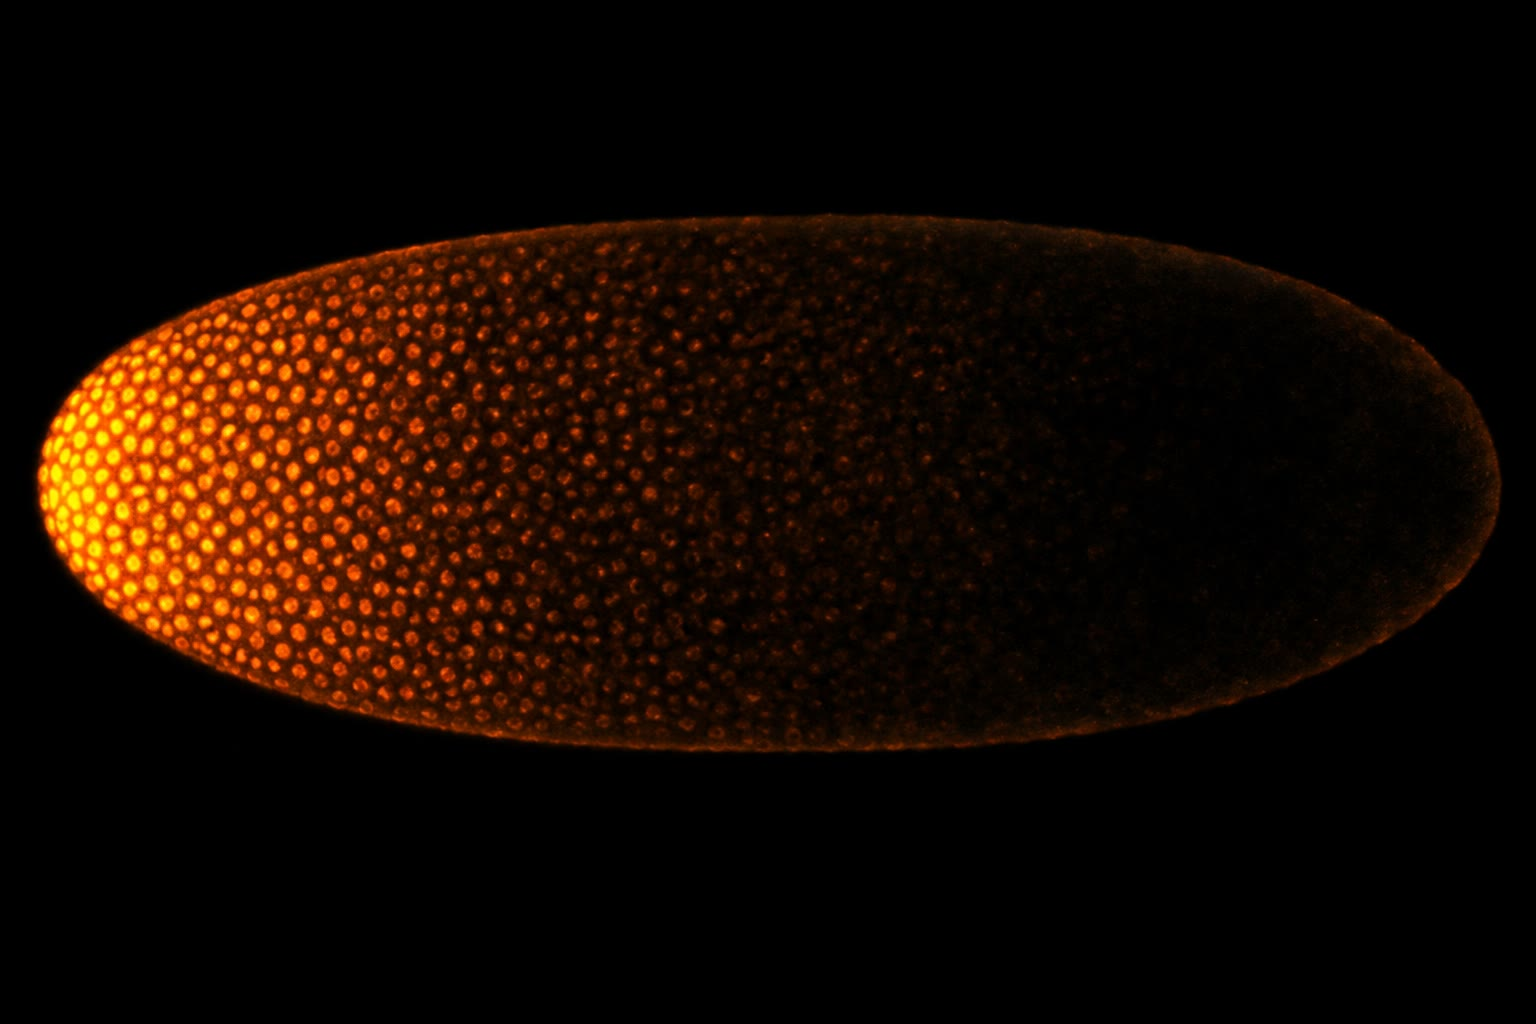
\includegraphics[width=0.46\linewidth]{images/book5/ai/b5-23-bicoid-gradient.jpg}\hspace{0.04\linewidth}
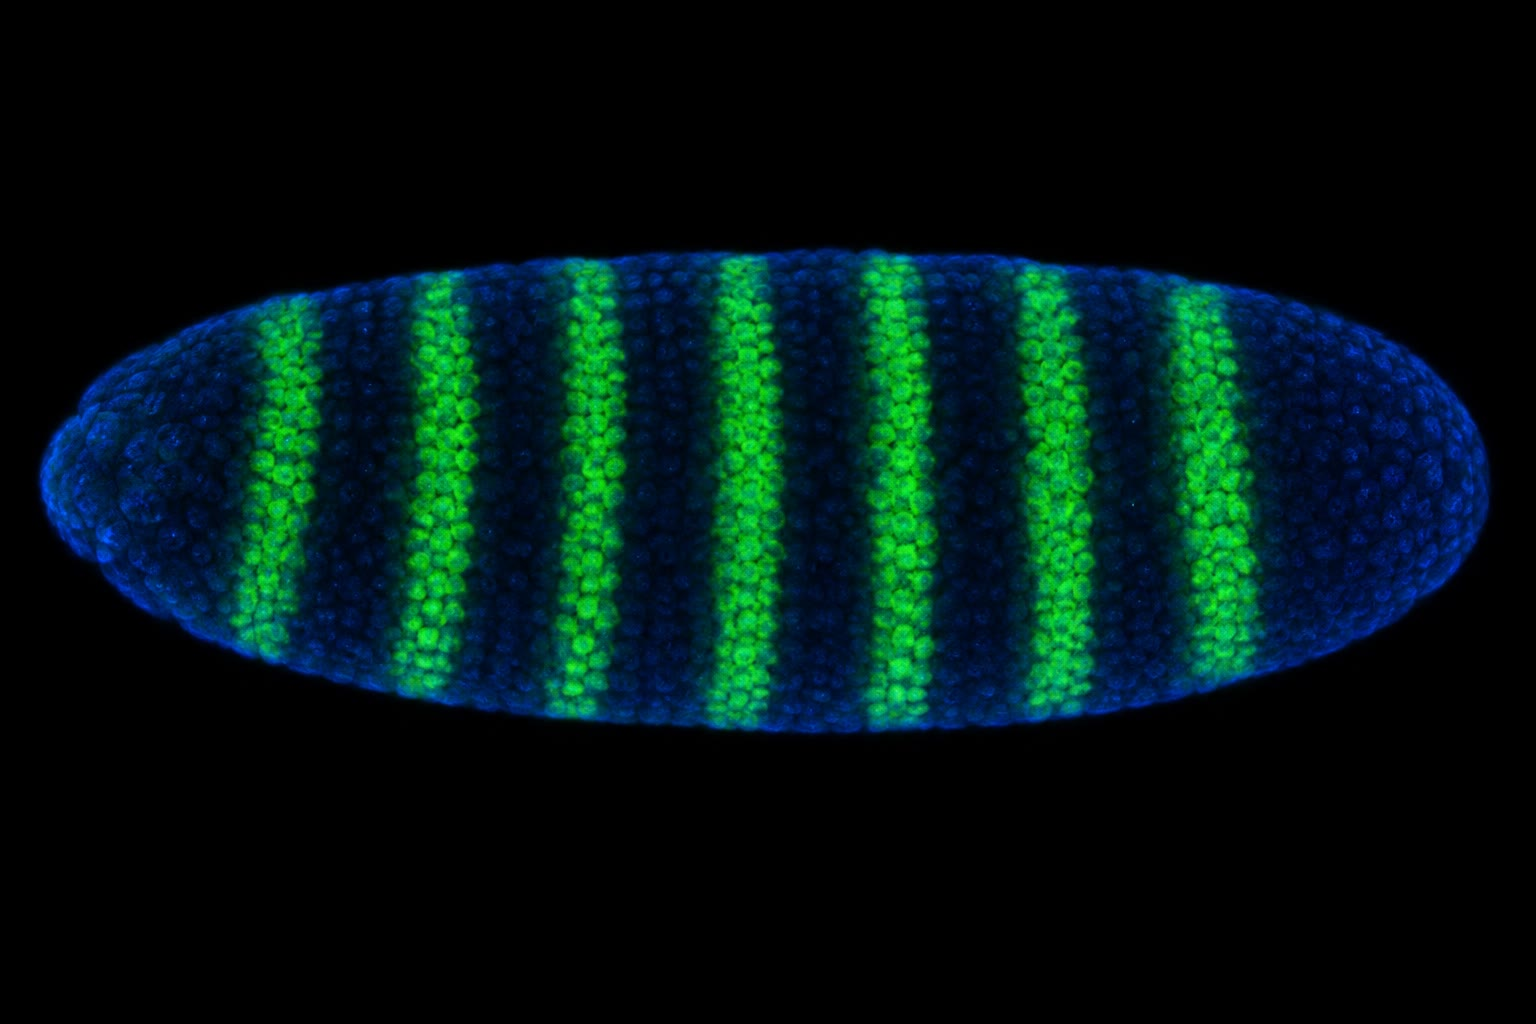
\includegraphics[width=0.46\linewidth]{images/book5/ai/b5-23-embryo-stripes.jpg}

{\small يسارًا: جنين مدمج مصبوغ لبروتين Bicoid، أشدّ سطوعًا
عند القطب الأمامي ويخفت أسّيًا نحو الخلف. ويمينًا: جنين بعد
ساعة مصبوغ لبروتين زوجي القاعدة، وسبعة خطوط مرسومة من
الأشرطة المورّثية الفجوية.}
\end{omfigure}

\section{الهوية: مورّثات Hox}

\begin{definition}[المورّثات الهوميوتية والتوافق الخطي]\label{def:b3:developmental-genetics:hox}
\index{طفرة هوميوتية}\index{مورّثات Hox}\index{توافق خطي}\index{هوميوبوكس}\index{شفرة Hox}
الطفرة \emph{الهوميوتية} تحوّل جزءًا من الجسم إلى آخر: وهي
كلمة بيتسون (1894) للشذوذات التي ``تُحلّ عضوًا من سلسلة محل
آخر''. ففي الذبابة، تنمي طافرات \emph{Antennapedia} السائدة
أرجلًا حيث ينبغي أن تكون قرون الاستشعار؛ وتحوّل طافرات
\emph{bithorax} (لويس، 1978) القطعة الصدرية الثالثة إلى نسخة
من الثانية، فتصير الموازنات (الدبوسيات) زوجًا ثانيًا من
الأجنحة. والمورّثات الثماني المسؤولة، وهي \emph{مورّثات Hox}،
تقع في عنقودين على صبغي واحد، ولاحظ لويس أن ترتيبها على
امتداد DNA يطابق ترتيب القطع التي تتحكم بها على امتداد الجسم
--- أي \emph{التوافق الخطي}، الذي لم يُفسَّر بعد تفسيرًا
تامًا. وترمّز كل منها عامل استنساخ بنطاق \emph{الهوميوبوكس}
نفسه الرابط لجزيء DNA والمؤلَّف من ستين حمضًا أمينيًا (مكغينيس،
وغيرنغ، 1984)، وقد وُجد بعد ذلك في كل حيوان: فللفئران
والبشر أربعة عناقيد من ثلاث عشرة مورّثة لكل عنقود، متوافقة
خطيًا بالطريقة نفسها، معبَّرًا عنها في نطاقات متداخلة على
امتداد محور الجسم، والمورّثات المتأخرة في العنقود أكثر
خلفيةً. وهوية الخلية على امتداد المحور يعطيها توافيق مورّثات
Hox التي تعبّر عنها، أي \emph{شفرة Hox}؛ والمورّثات الخلفية
تغلب الأمامية (الغلبة الخلفية)، ففقد مورّثة خلفية يدع القطعة
تتخذ هوية التي أمامها. ومورّثات Hox لا تبني قطعة؛ بل تخبر
قطعة مبنيّة أصلًا أيَّ قطعة هي، بتشغيل بطاريات المورّثات
التالية المناسبة لرجل أو جناح أو ضلع أو فقرة قطنية.
\end{definition}

\begin{omfigure}
\begin{tikzpicture}[every node/.style={font=\scriptsize}, >=stealth]
  % fly cluster
  \node[left] at (-0.3,2.2) {الذبابة (\emph{Drosophila})، 8 مورّثات};
  \foreach \i/\g/\c in {0/lab/omDef, 1/pb/omDef, 2/Dfd/omThm, 3/Scr/omThm, 4/Antp/omMeth, 5/Ubx/omMeth, 6/abd-A/omProp, 7/Abd-B/omProp} {
    \draw[thick, fill=\c!40] ({\i*1.1},1.9) rectangle ({\i*1.1+0.9},2.5); \node[font=\tiny] at ({\i*1.1+0.45},2.2) {\emph{\g}};
  }
  \node[left] at (-0.3,0.9) {عنقود HoxB في الفأر، 9 من 13};
  \foreach \i/\g/\c in {0/b1/omDef, 1/b2/omDef, 2/b3/omDef, 3/b4/omThm, 4/b5/omThm, 5/b6/omMeth, 6/b7/omMeth, 7/b8/omProp, 8/b9/omProp} {
    \draw[thick, fill=\c!40] ({\i*1.1},0.6) rectangle ({\i*1.1+0.9},1.2); \node[font=\tiny] at ({\i*1.1+0.45},0.9) {\emph{\g}};
  }
  \draw[->, thick] (0,1.55) -- (9.8,1.55); \node[above, font=\tiny] at (4.9,2.55) {3$'$ $\to$ 5$'$ على امتداد DNA};
  \draw[->, thick] (0,0.2) -- (9.8,0.2); \node[below, font=\tiny] at (4.9,0.05) {الأمام $\to$ الخلف على امتداد الجسم};
  % body schematic
  \node[left] at (-0.3,-0.9) {يُعبَّر عنها في};
  \draw[thick, gray!70, rounded corners=6pt] (0,-1.3) rectangle (9.8,-0.5);
  \foreach \x/\t in {0.6/رأس, 2.6/عنق, 4.4/صدر, 6.6/قطني, 8.6/{عجزي، وذنب}} { \node[font=\tiny] at (\x,-0.9) {\t}; }
  \draw[gray!70] (1.6,-1.3) -- (1.6,-0.5); \draw[gray!70] (3.5,-1.3) -- (3.5,-0.5); \draw[gray!70] (5.6,-1.3) -- (5.6,-0.5); \draw[gray!70] (7.6,-1.3) -- (7.6,-0.5);
  \node[below, align=center, font=\tiny] at (4.9,-1.4) {التوافق الخطي: ترتيب المورّثات على الصبغي هو ترتيب نطاقاتها على امتداد الجسم؛\\العناقيد نفسها، والترتيب نفسه، من الذبابة إلى الفأر ---\\موروثة من سلف قبل 600 مليون سنة};
\end{tikzpicture}

{\small عنقودا Hox في ذبابة وفأر. تقع المورّثات على امتداد
DNA بترتيب مناطق الجسم التي تحددها، في الحيوانين معًا،
والمورّثات المتماثلة تُعرف بالتسلسل: فمورّثة \emph{Hoxb6} في
الفأر هي بوضوح \emph{Antennapedia} الذبابة.}
\end{omfigure}

\begin{proof}[شواهد]
رسم لويس (1978) خريطة معقد \emph{bithorax} سلسلةً من الطفرات
تحوّل كل واحدة قطعةً إلى التي أمامها، مرتبةً على الصبغي
بترتيب الجسم، واقترح أن المورّثات تُفعَّل تتابعًا على امتداد
المحور. ووجد مكغينيس وزملاؤه (1984) \omterm{def:b3:developmental-genetics:hox}{الهوميوبوكس} بالتهجين
المتصالب بين \emph{Antennapedia} و\emph{Ultrabithorax} ثم في
الضفادع والفئران. وأما التكافؤ الوظيفي فقد بُيّن مباشرةً:
فمورّثة \emph{Hoxb6} من الفأر معبَّرًا عنها في ذبابة تنتج
النمط الظاهري \emph{Antennapedia}، أي أرجلًا من قرون
الاستشعار (في تسعينيات القرن العشرين)؛ وفأر يفتقر إلى
\emph{Hoxc8} له ضلع إضافي على فقرته القطنية الأولى، إذ اتخذت
القطعة هوية التي أمامها؛ وتغييرُ حدود تعبير Hox في الكتكوت
والفأر يزيح الموضع الذي تتكوّن فيه الأطراف الأمامية، وطولُ
عنق البجعة يقابله انزياح خلفي للحد نفسه.
\end{proof}

\begin{omfigure}
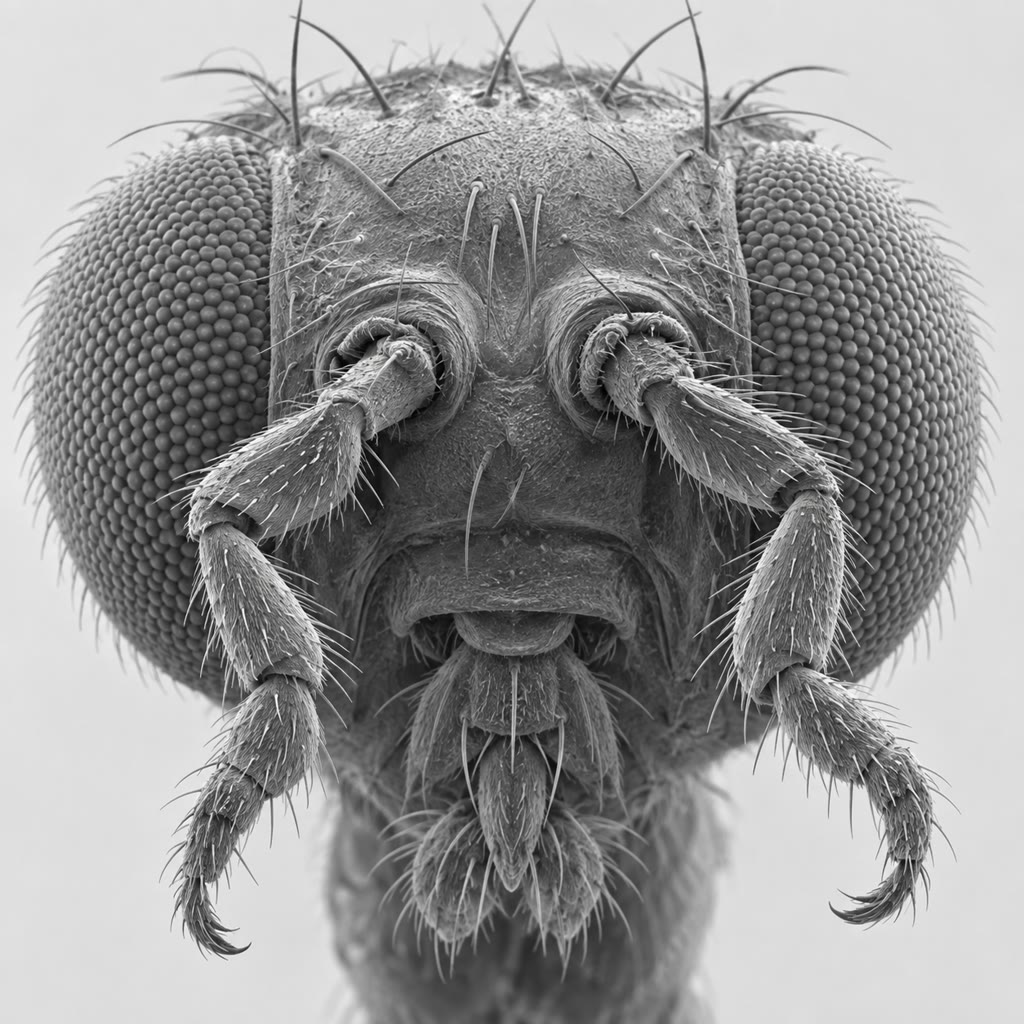
\includegraphics[width=0.34\linewidth]{images/book5/ai/b5-23-antennapedia-fly.jpg}\hspace{0.04\linewidth}
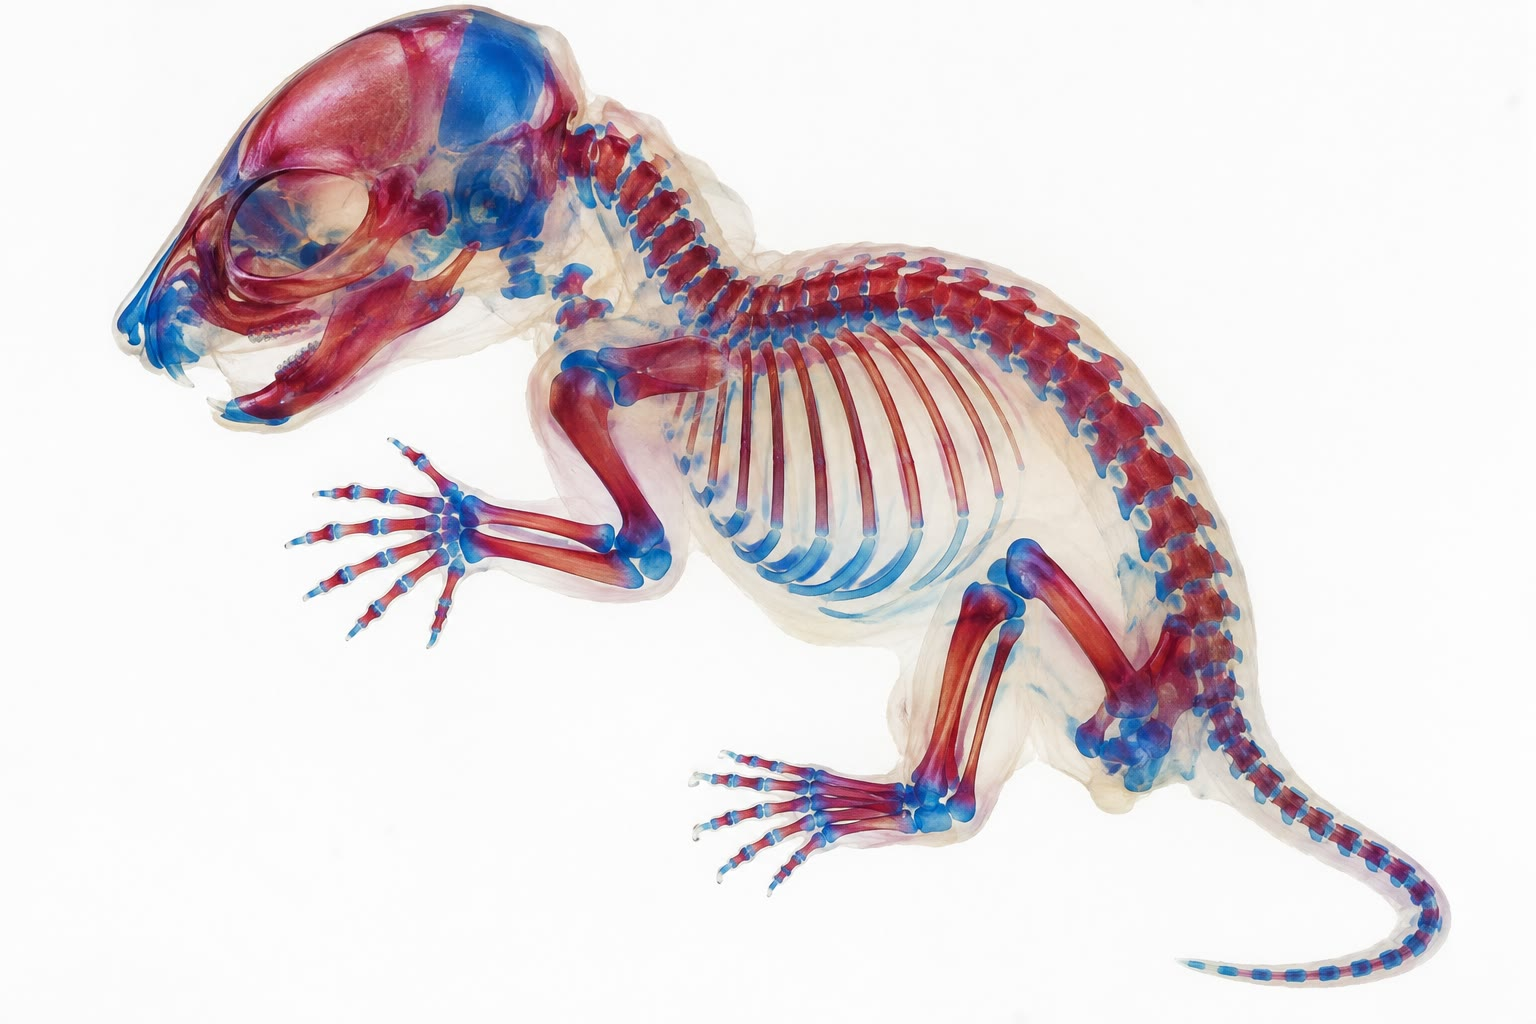
\includegraphics[width=0.5\linewidth]{images/book5/ai/b5-23-limb-skeleton-stain.jpg}

{\small يسارًا: رأس ذبابة طافرة \emph{Antennapedia}، وزوج من
الأرجل حيث ينبغي أن تكون قرون الاستشعار --- فالقطعة بُنيت
بناءً صحيحًا وأُخبرت بالهوية الخطأ. ويمينًا: هيكل جنين فأر،
الغضروف أزرق والعظم أحمر، والفقرات التي تُقرأ عليها \omterm{def:b3:developmental-genetics:hox}{شفرة Hox}.}
\end{omfigure}

\section{بناء فقاري}

\begin{definition}[المنظِّمات ومراكز الإشارة]\label{def:b3:developmental-genetics:organiser}
\index{منظِّم}\index{استحثاث}\index{sonic hedgehog}\index{برعم الطرف}\index{منطقة النشاط المستقطِب}\index{عرف أديمي ظاهر قمي}
أجنّة الفقاريات خلوية من البداية، فتصنع تدرجاتها ببروتينات
مفرَزة لا بانتشار في مدمج، وتفعل بضع العائلات نفسها كل شيء:
Wnt، وHedgehog، وBMP وسائر أقارب TGF-$\beta$،
وFGF، وNotch، وحمض الريتينويك. وقد طعّم شبيمان ومانغولد (1924)
قطعةً من الشفة الظهرية لمعيدة سمندر على بطن أخرى فحصلا على
جنين ثانٍ، من الرأس إلى الذنب، مصنوع في معظمه من خلايا
المضيف: فقد كان الطعم \emph{منظِّمًا}، يستحث جيرانه على
تكوين جهاز عصبي ومحور، ووُجدت جزيئاته بعد سبعين سنة مضادات
مفرَزة (الكوردين، والنوغين) تحجب BMP، الذي يدع غيابه الأديم
الظاهر يصير عصبيًا --- وهو الوضع الافتراضي.
و\emph{الأنبوب العصبي} يُنمَّط بعد ذلك ظهريًا بطنيًا بالبروتين \emph{sonic
hedgehog} من الحبل الظهري والصفيحة القاعدية (مرتفعًا:
عصبونات حركية؛ منخفضًا: عصبونات بينية) في مواجهة BMP من
السقف؛ و\emph{برعم الطرف} يُنمَّط بمركزين، هما \emph{منطقة
النشاط المستقطِب} عند حافته الخلفية وهي تفرز Shh (وطعمها إلى
الحافة الأمامية يعطي مضاعفةً مرآتية للأصابع، ستة أصابع
يلتقي إبهامان في وسطها) و\emph{العرف الأديمي الظاهر القمي}
عند طرفه وهو يفرز FGF التي تبقي الخلايا تحته منقسمة وتحدد
التتابع من القريب إلى البعيد: العضد، والساعد، واليد.
والتطعيم والاستئصال والحبيبات المشبعة بالبروتين تبقى
الأدوات؛ وأما المنطق --- منبع موضعي، وتدرج، وعتبات، وشفرة من
عوامل الاستنساخ --- فهو منطق الذبابة.
\end{definition}

\begin{omfigure}
\begin{tikzpicture}[every node/.style={font=\scriptsize}, >=stealth]
  % limb bud
  \fill[omDef!12] (0,0) -- (0,3) .. controls (2.6,3.4) and (3.4,2.2) .. (3.4,1.5) .. controls (3.4,0.8) and (2.6,-0.4) .. (0,0) -- cycle;
  \draw[thick, omDef] (0,0) -- (0,3) .. controls (2.6,3.4) and (3.4,2.2) .. (3.4,1.5) .. controls (3.4,0.8) and (2.6,-0.4) .. (0,0);
  \draw[very thick, omMeth!70!black] (2.9,2.5) .. controls (3.45,1.9) and (3.45,1.1) .. (2.9,0.5);
  \node[right, align=left, omMeth!70!black, font=\tiny] at (3.5,1.5) {العرف الأديمي الظاهر القمي:\\FGF8؛ يبقي منطقة\\التقدم منقسمة؛\\من القريب $\to$ إلى البعيد};
  \begin{scope}
    \clip (0,0) -- (0,3) .. controls (2.6,3.4) and (3.4,2.2) .. (3.4,1.5) .. controls (3.4,0.8) and (2.6,-0.4) .. (0,0) -- cycle;
    \foreach \i/\op in {1/50, 2/38, 3/26, 4/14} { \draw[omThm!\op, thick] (0.6,0.5) circle ({0.45*\i}); }
  \end{scope}
  \fill[omThm!50] (0.6,0.5) ellipse (0.5 and 0.35); \node[anchor=north, align=center, omThm, font=\tiny] at (0.9,-0.2) {منطقة النشاط المستقطِب: sonic hedgehog،\\من الخلف $\to$ إلى الأمام};
  \node[left, font=\tiny] at (-0.05,2.6) {الأمام}; \node[left, font=\tiny] at (-0.05,0.4) {الخلف};
  \node[left, font=\tiny] at (-0.05,1.5) {جدار الجسم};
  \draw[->, thick] (0.3,1.5) -- (3.0,1.5); \node[above, font=\tiny] at (1.75,1.55) {العضد، والساعد، والأصابع};
  % right: digit code
  \node[right, align=left] at (7.2,2.6) {هوية الإصبع من التعرض للبروتين Shh:\\الإبهام (الإصبع 1): لا تعرض؛\\والإصبعان 2--3: تدرج؛\\والإصبعان 4--5: من خلايا تعبّر عن Shh};
  \node[right, align=left] at (7.2,1.0) {اطعم منطقة نشاط مستقطِب ثانية أماميًا:\\مضاعفة مرآتية، 4-3-2-2-3-4؛\\وحبيبة من بروتين Shh تفعل الشيء نفسه};
  \node[right, align=left, gray] at (7.2,-0.2) {الجزيء نفسه ينمّط الأنبوب العصبي\\(العصبونات الحركية حيث يرتفع) والمعي};
\end{tikzpicture}

{\small مركزا الإشارة في \omterm{def:b3:developmental-genetics:organiser}{برعم الطرف}. يخبر \omterm{def:b3:developmental-genetics:organiser}{sonic hedgehog} من
الحافة الخلفية الخلايا أي إصبع تصير؛ ويخبرها FGF من الطرف كم
بعدت على امتداد الطرف. والطعوم التي تنقل مركزًا تنقل النمط
معه.}
\end{omfigure}

\begin{proposition}[نمط عفوي: آلية تورنغ]\label{prop:b3:developmental-genetics:turing}
\index{نمط تورنغ}\index{تفاعل--انتشار}\index{منشِّط--مثبِّط}
ليس كل نمط مقروءًا من تدرج سابق. فقد بيّن تورنغ (1952) أن
مادتين منتشرتين تتفاعلان --- \emph{منشِّط} يحفّز إنتاج نفسه
وإنتاج \emph{مثبِّط}، ومثبِّط يكبت المنشِّط وينتشر أسرع منه
بكثير --- تقدران على تحويل حقل منتظم إلى مصفوفة منتظمة من
الذرى عفويًا: فزيادة موضعية صغيرة من المنشِّط تنمو بالتعزيز
الذاتي بينما ينتشر المثبِّط الذي تنتجه ويمنع تكوّن ذرى
جديدة قربها، فتظهر الذرى بتباعد يحدده مدى المثبِّط،
$\lambda \sim \sqrt{D_{\text{inh}}/k_{\text{inh}}}$،
لا أي إحداثي خارجي. والآلية، المسلَّم بها هنا في رياضياتها،
أفضل تفسير لبقع معاطف الحيوانات وخطوطها، ولتباعد جُريبات
الشعر وبراعم الريش، ولحُرُف الحنك، ولأصابع اليد (التي يرتفع
عددها حين يُقصَّر طول موجة النمط بخفض فعالية Hox)، ولخطوط
سمك الزرد، حيث عُيّنت الخلايا المتفاعلة --- خلايا صبغية
تنفر من جاراتها من صنف وتجذب من صنف آخر عن بُعد --- وجُعلت
خطوطها تتكوّن من جديد بعد استئصال بالليزر تمامًا كما تتنبأ
النظرية.
\end{proposition}
\admitted

\section{تطور الشكل}

\begin{definition}[التطور والنماء]\label{def:b3:developmental-genetics:evodevo}
\index{تماثل عميق}\index{عدّة مورّثية}\index{تطور تنظيمي جانبي}\index{اختلاف التوقيت}
المورّثات التي تبني الحيوانات \emph{عدّة} قديمة مشتركة: بضع
مئات من عوامل الاستنساخ وسبل الإشارة الحاضرة في السلف
المشترك للحيوانات جميعًا، وتنوع الحيوانات يأتي في معظمه من
تغيّرات في \emph{متى وأين وبكم} يُعبَّر عنها لا فيما ترمّزه.
فأما \emph{التماثل العميق}: فالمورّثة \emph{Pax6} توجّه تكوين
العين في الذباب والحبار والفئران، وأعينها ليست متماثلة
أعضاءً --- ومورّثة \emph{Pax6} من فأر معبَّرًا عنها على رجل
ذبابة تصنع عين ذبابة في غير موضعها هناك (هالدر، وغيرنغ،
1995). وأما \emph{التطور التنظيمي الجانبي}: ففقدُ الأشواك
الحوضية في شوكيات الظهر العذبة حذفُ معزِّز واحد للمورّثة
\emph{Pitx1}، والبروتين سليم ولا يزال يخدم في مواضع أخرى؛
وفقدُ بقع الجناح في بعض ذباب الفاكهة تغيّرٌ في معزِّز
\emph{yellow}؛ وفقدُ الأرجل في الأفاعي معزِّزٌ مكسور لمورّثة
\emph{\omterm{def:b3:developmental-genetics:organiser}{sonic hedgehog}} في الطرف. وأما \emph{انزياحات Hox}:
فحدّ تعبير \emph{Hoxc6} يعلّم الفقرة الصدرية الأولى في الفأر
والكتكوت والإوزة والأفعى سواءً، عند الفقرة 7 و14 و23 و3؛
وفقدُ الحشرات أرجلها البطنية كان اكتساب البروتين Ubx نطاقًا
كابتًا يطفئ مورّثة الرجل \emph{Distal-less}، حيث لا يفعل ذلك
في القشريات. وأما \emph{اختلاف التوقيت}، وهو تغيّر في توقيت
برنامج نمائي، فقد جعل الأكسولوتل يرقةً دائمة وجعل وجه
الإنسان وجه قرد يافع. والسؤال القديم عن كيف تنشأ أشكال
جديدة يصير سؤالًا عن DNA التنظيمي: فمعظم الجينوم الذي يهم
الشكل ليس مورّثة بل مفتاحًا.
\end{definition}

\begin{example}[أربعة أجنحة]\label{ex:b3:developmental-genetics:four-wings}
كان لأسلاف الذباب أربعة أجنحة، كما لا يزال لليعاسيب والنحل؛
وللذباب اثنان، والزوج الخلفي مختزل إلى موازنات. ففي الذباب
يُعبَّر عن \emph{Ultrabithorax} في القطعة الصدرية الثالثة
ويكبت برنامج الجناح هناك --- أي نحو مئة مورّثة هدف، فالدبوسية
جناح أُطفئت تلك المورّثات فيه. وذبابة لويس الثلاثية الطفرة،
الفاقدة لوظيفة \emph{Ubx} في القطعة الثالثة، تنمي زوجًا
ثانيًا من الأجنحة: لا بنيةً جديدة بل إطلاق بنية قديمة. وفي
الفراشات يُعبَّر عن \emph{Ubx} في الجناح الخلفي أيضًا، وهو
لا يكبت الجناح هناك بل يغيّر نمطه: فالبروتين نفسه، ومجموعة
أهداف مختلفة. فأربعمئة مليون سنة من تطور ثنائيات الأجنحة
توقفت على قرار مورّثة واحدة في قطعة واحدة، وطفرة واحدة تنقضه
في جيل --- ولذلك يكون تاريخ الشكل مقروءًا في المورّثات التي
تبنيه.
\end{example}

\begin{remark}[هندسة من كيمياء]\label{rem:b3:developmental-genetics:remark}
ليس للجنين مخطط ولا مسّاح. وإنما له بضعة تدرجات يصنعها
الانتشار والاضمحلال، وخلايا تقرؤها في مواجهة عتبات وتشغّل
عوامل استنساخ، وشفرة من تلك العوامل تخبر كل منطقة بما تصير؛
وله منظِّمات موضعية تستحث جيرانها، وتفاعلات تنمّط نفسها.
والرياضيات رياضيات الحركيات من الرتبة الأولى والانتشار ---
أسّي، وجذر تربيعي، وعتبة --- وهي تفسر لا كيف يوضع رأس ذبابة
فحسب، بل لماذا تزيح مضاعفةُ مورّثة حدًّا مسافة ثابتة، ولماذا
تظهر ستة أصابع حين تُضاعف إشارة، ولماذا للأفعى ثلاثمئة ضلع.
فالتطور يحرّر المفاتيح، لا الآلة: فعدّة الإسفنجة والإنسان
تكاد تكون واحدة، والذي يختلف هو التوصيل.
\end{remark}

\section{تمارين}

\begin{exercise}[$\star$]\label{exo:b3:developmental-genetics:1}
سمّ طبقات تراتب التقطيع الأربع في الذبابة، ومورّثة من كل
طبقة، والنمط الظاهري الطافر الذي وضعها في صنفها.
\end{exercise}

\begin{exercise}[$\star$]\label{exo:b3:developmental-genetics:2}
ما \omterm{def:b3:developmental-genetics:hierarchy}{مورّثة الأثر الأمومي}؟ أنثى متخالصة الزيجة لطفرة عديمة في
\emph{bicoid} تُزاوَج بذكر بري: صف أجنّتها واشرح لماذا لا
ينقذها نمطها الوراثي هي.
\end{exercise}

\begin{exercise}[$\star$]\label{exo:b3:developmental-genetics:3}
اذكر \omterm{def:b3:developmental-genetics:hox}{التوافق الخطي} والغلبة الخلفية. وتنبأ بالنمط الظاهري
لفأر يفتقر إلى \emph{Hoxc8} ولذبابة تعبّر عن
\emph{Antennapedia} في رأسها.
\end{exercise}

\begin{exercise}[$\star$]\label{exo:b3:developmental-genetics:4}
ماذا أظهر طعم شبيمان ومانغولد، وأي جزيئات تبيّن أنها جزيئات
\omterm{def:b3:developmental-genetics:organiser}{المنظِّم}؟ ولماذا يُسمّى المصير العصبي ``الافتراضي''؟
\end{exercise}

\begin{exercise}[$\star\star$]\label{exo:b3:developmental-genetics:5}
لبروتين Bicoid: $D = \qty{4}{\micro m^2/s}$، وعمر نصف
\qty{35}{min}. احسب $k$، و$\lambda$، ونسبة التركيزين عند
القطب الأمامي وعند منتصف البيضة (\qty{250}{\micro m}).
\end{exercise}

\begin{exercise}[$\star\star$]\label{exo:b3:developmental-genetics:6}
عند $\lambda = \qty{100}{\micro m}$، يقع حدّ عند
\qty{240}{\micro m}. فأين يقع إذا حملت الأم أربع نسخ من
\emph{bicoid} بدل نسختين؟ وإذا حملت نسخة واحدة؟ عبّر عن
الإزاحتين نسبةً إلى بيضة طولها \qty{500}{\micro m}.
\end{exercise}

\begin{exercise}[$\star\star$]\label{exo:b3:developmental-genetics:7}
تتباعد النُوى في الأديم الأرومي \qty{8}{\micro m}. فلوضع حدّ
في حدود نواة واحدة عند $\lambda = \qty{100}{\micro m}$، بأي
دقة يجب أن تقرأ النواة تركيز Bicoid؟ وإذا عدّت النواة
الجزيئات على مدى زمن $\tau$ وكان العدّ بواسونيًا، فكم يجب أن
تعدّ؟
\end{exercise}

\begin{exercise}[$\star\star$]\label{exo:b3:developmental-genetics:8}
يقترب التدرج من الحالة المستقرة على المقياس الزمني $1/k$.
فعند عمر نصف قدره \qty{35}{min}، أي نسبة من تركيز الحالة
المستقرة تُبلَغ عند \qty{60}{min}، و\qty{90}{min}، و\qty{120}{min}؟
وبماذا يقتضي ذلك لجنين عليه أن يقرأ التدرج عند \qty{150}{min}؟
\end{exercise}

\begin{exercise}[$\star\star$]\label{exo:b3:developmental-genetics:9}
تُطعَّم منطقة نشاط مستقطِب إلى الحافة الأمامية لبرعم طرف
كتكوت. تنبأ بنمط الأصابع، وبالنمط لو زُرعت هناك بدل ذلك
حبيبة تطلق جرعة منخفضة من Shh.
\end{exercise}

\begin{exercise}[$\star\star\star$]\label{exo:b3:developmental-genetics:10}
يُصنع مورفوجين في نسيج طوله $L$ كله بمعدل $s$ في وحدة الحجم،
ويُهدم بمعدل $k$، ويُتلف عند الحد $x =
L$ (بالوعة ماصّة)، بلا دفق عند $x = 0$. حلّ $Dc'' - kc + s =
0$ من أجل $c(x)$ وارسمه. وبم يختلف شكل هذا التدرج عن حالة
المنبع عند طرف واحد، وماذا يحدث حين $L \ll \lambda$؟
\end{exercise}

\begin{exercise}[$\star\star\star$]\label{exo:b3:developmental-genetics:11}
عتبتان عند $T_{1} = 0.3c_{0}$ و$T_{2} = 0.08c_{0}$ تقسمان
تدرجًا إلى ثلاث مناطق. بيّن أن عرضي المنطقتين الأوليين لا
يتوقفان على $c_{0}$، واشرح لماذا يحتاج جنين يتباين \emph{طوله}
بين الأفراد (من \qty{450}{} إلى \qty{550}{\micro m}) إلى ما هو
أكثر من أسّي واحد ليدرّج نمطه. واقترح آلية واحدة.
\end{exercise}

\begin{exercise}[$\star\star\star$]\label{exo:b3:developmental-genetics:12}
فقدت شوكيات الظهر أشواكها الحوضية بحذف معزِّز للمورّثة \emph{Pitx1}،
وفقدت الأفاعي أطرافها بكسر معزِّز للمورّثة \emph{\omterm{def:b3:developmental-genetics:organiser}{sonic hedgehog}}.
اشرح لماذا تكون التغيّرات التنظيمية لا الترميزية هي الطريق
المعتاد إلى بنية مفقودة أو متبدلة، من حيث تعدد الأثر ومن حيث
ما يفعله البروتين نفسه في مواضع أخرى.
\end{exercise}

\section{مسألة: العلم الفرنسي}

\begin{problem}[{مسألة نهاية الأسبوع --- جملة إحداثيات بيضة
تُحسب من حركيات الرتبة الأولى: طول تدرج Bicoid، ومنبعه، وزمن
تكوّنه، والحدود التي يرسمها ودقتها، وما تفعله جرعة المورّثة
وحجم البيضة بها، وشفرة Hox المقروءة بعدها، وتُختم بطول
الاضمحلال، وبالإزاحة لكل مضاعفة، وبالدقة الموضعية}]
\label{pb:b3:developmental-genetics:1}
المعطيات: طول البيضة \qty{500}{\micro m}؛ ولبروتين Bicoid $D = \qty{4}{\micro m^2/s}$،
وعمر نصف \qty{35}{min}؛ ودفق منبع بحيث يكون $c_{0} = \qty{50}{nM}$
مع نسختين أموميتين؛ وتباعد النُوى \qty{8.5}{\micro m} في الدورة
14؛ والعتبتان $T_{1} = 0.3\,c_{0}$ (الرأس/الصدر) و$T_{2} =
0.08\,c_{0}$ (حدّ \emph{hunchback}) في حالة النسختين. وضجيج
القراءة $\delta c/c = 0.1$ للنواة الواحدة. وعدد أفوغادرو
\qty{6e23}{}؛ والنواة كرة نصف قطرها \qty{3}{\micro m}.

\medskip
\noindent\textbf{الجزء الأول --- التدرج.}
\begin{enumerate}
  \item احسب $k$ من عمر النصف، بوحدة \unit{s^{-1}}، والعمر
        $1/k$ بالدقائق.
  \item احسب $\lambda = \sqrt{D/k}$ بالميكرومترات. وكم طول
        اضمحلال تساوي البيضة؟
  \item بأي عامل يهبط التركيز من قطب إلى قطب؟ وبأي عامل على
        امتداد تباعد نووي واحد عند منتصف البيضة؟
  \item احسب دفق المنبع $J = c_{0}\sqrt{Dk}$ بوحدة
        \unit{nM\,\micro m\,s^{-1}}، وعدد الجزيئات الداخلة إلى
        رقعة \qty{1}{\micro m^2} من القطب الأمامي في الثانية.
  \item عدد جزيئات Bicoid في نواة عند القطب (عند $c_{0}$)
        وعند منتصف البيضة.
  \item النسبة المبلوغة من الحالة المستقرة عند \qty{60}{min}
        وعند \qty{120}{min} ($1 - \mathrm{e}^{-kt}$). فهل يكون
        التدرج مستقرًا حين تُرسم الحدود، عند نحو \qty{120}{min}؟
\end{enumerate}

\medskip
\noindent\textbf{الجزء الثاني --- الحدود.}
\begin{enumerate}[resume]
  \item موضعا الحدين، بوحدة \unit{\micro m} وكنسبتين من طول
        البيضة.
  \item للأم أربع نسخ: فما $c_{0}$ الجديد، وما موضعا الحدين؟
        وبكم تحرك كل منهما؟ وست نسخ؟
  \item نسخة واحدة: المواضع. وأي المناطق كبرت وأيها صغرت؟
  \item الخطأ الموضعي عن ضجيج قراءة قدره \qty{10}{\%}،
        بالميكرومترات وبالتباعدات النووية.
  \item إذا وجب أن يكون الخطأ نواةً واحدة، فأي دقة قراءة
        تلزم؟ وإذا توسطت النواة $n$ قراءة مستقلة وهبط الضجيج
        بالمقدار $1/\sqrt{n}$، فكم قراءة تلزم؟
  \item نواة عند حدّ \emph{hunchback} تحوي العدد المحسوب في
        السؤال~5. فما ضجيج بواسون $1/\sqrt{N}$ لعدّة آنية
        واحدة؟ قارن ذلك بنسبة \qty{10}{\%} وعلّق.
\end{enumerate}

\medskip
\noindent\textbf{الجزء الثالث --- التدريج والمتانة.}
\begin{enumerate}[resume]
  \item تتباين البيوض من \qty{450}{} إلى \qty{550}{\micro m}.
        فإذا كان $\lambda$ و$c_{0}$ ثابتين، فأين يقع حدّ
        \emph{hunchback} كنسبة من طول البيضة في كل منهما؟ وهل
        يكون النمط مدرَّجًا؟
  \item افترض بدل ذلك أن $D$ يتدرج بالمقدار $L^{2}$ (العمر نفسه،
        لكن منبعًا ينمو انتشاره مع البيضة). بيّن أن
        $\lambda/L$ يكون عندئذ ثابتًا وأن النمط يتدرج. وهل
        ذلك معقول؟
  \item تستجيب المورّثة \emph{hunchback} لبروتين Bicoid بمعامل هِل
        قدره $5$: فتعبيرها $c^{5}/(c^{5} + T^{5})$. فعلى كم
        ميكرومترًا ينتقل التعبير من \qty{10}{\%} إلى
        \qty{90}{\%} حول الحد؟ وقارن ذلك بتباعد نووي واحد.
  \item اشرح لماذا تحدّ استجابةٌ حادّة حدًّا لكنها لا تخفض
        بنفسها الخطأ الموضعي الناشئ عن ضجيج التركيز.
  \item الكبت المتبادل بين المورّثات الفجوية يحدّ حدودها
        ويثبّتها. احتجّ في جملة واحدة لأن مورّثتين تكبت كل
        منهما الأخرى لا يمكن أن تكونا مشغَّلتين معًا في
        النواة نفسها في الحالة المستقرة.
  \item ترفع الحرارة $D$ بمقدار \qty{2}{\%} و$k$ بمقدار
        \qty{6}{\%} لكل درجة. فما التغيّر في $\lambda$ لكل
        درجة، وما إزاحة الحد في غرفة أدفأ بمقدار \qty{5}{\celsius}؟
        ولماذا قد تحتاج الأجنّة إلى آلية معوِّضة؟
\end{enumerate}

\medskip
\noindent\textbf{الجزء الرابع --- الهوية.}
\begin{enumerate}[resume]
  \item \omterm{def:b3:developmental-genetics:hox}{شفرة Hox}: مع ثماني \omterm{def:b3:developmental-genetics:hox}{مورّثات Hox} في الذبابة كل واحدة
        مشغَّلة أو مطفأة، كم شفرة ممكنة؟ وكم منها مستعملة
        (أربع عشرة قطعة)؟ ولماذا تخفض الغلبة الخلفية العدد
        الفعال؟
  \item ذبابة تفتقر إلى \emph{Ubx} في قطعتها الصدرية الثالثة.
        فماذا تصير القطعة، ولماذا تكون النتيجة أربعة أجنحة لا
        بنية جديدة؟
  \item يقع حدّ \emph{Hoxc6} في الفأر عند الفقرة 7 وفي الإوزة
        عند 23. فبماذا يتنبأ ذلك عن عنقيهما، وما الذي تغيّر
        في التطور: المورّثة أم تعبيرها؟
  \item طعمُ منطقة نشاط مستقطِب يعطي الأصابع 4-3-2-2-3-4.
        اشرح النمط من تدرجي Shh يلتقيان في الوسط.
  \item عبّر هالدر وغيرنغ عن \emph{Pax6} الفأر في رجل ذبابة
        فحصلا على عين ذبابة هناك. فبماذا يدل ذلك عن المورّثة،
        وبماذا \emph{لا} يدل عن عيني الذباب والفئران؟
  \item الإصبع السادس: تقصير طول موجة تورنغ يضيف إصبعًا. فمع
        خمسة أصابع على امتداد صفيحة يد عرضها \qty{2}{mm}، أي
        تغيّر في طول الموجة يعطي ستة؟ وأي مُعامل في جملة
        التفاعل والانتشار ينتجه؟
  \item لخّص: قيمة $\lambda$ (السؤال~2)، وإزاحة الحد لكل
        مضاعفة للمنبع (السؤال~8)، والخطأ الموضعي عن ضجيج
        \qty{10}{\%} (السؤال~10).
\end{enumerate}
\end{problem}
